\subsection{Xây dựng mô hình hồi quy đa biến}

\textbf{Mục tiêu:} Định lượng sức tác động của các thông số kỹ thuật đến \texttt{Pixel\_Rate}.

\textbf{Phương trình tổng quát:} Trình bày phương trình hồi quy đa biến có lấy logarit để tuyến tính hóa quan hệ:
\begin{equation}
    \ln(\text{Pixel\_Rate}) = \beta_0 + \beta_1 \ln(X_1) + \beta_2 \ln(X_2) + \dots + \beta_n \ln(X_n) + \epsilon
\end{equation}

\subsubsection{Xây dựng mô hình 1 (Nvidia - GDDR - Resolution Group 1)}

\textbf{Lập luận tiền xử lý:} Tập dữ liệu được phân chia thành tập Huấn luyện (Train) và tập Kiểm tra (Test) theo tỷ lệ 2:1. Sau đó tiến hành kiểm tra đa cộng tuyến (\textbf{VIF}). Các biến gây nhiễu và làm sai lệch hệ số ($\text{VIF} > 5$) sẽ được xem xét loại bỏ. Thuật toán \textbf{Stepwise Selection} được áp dụng tuần tự nhằm tìm ra mô hình tối ưu nhất thông qua việc giảm thiểu chỉ số AIC.

\textbf{Kết quả thực nghiệm:}
\begin{center}
\begin{minipage}{0.85\textwidth}
\begin{mdframed}
\begin{verbatim}
Call:
lm(formula = as.formula(formula_str), data = data)

Residuals:
     Min       1Q   Median       3Q      Max 
-0.61049 -0.07799 -0.02266  0.03643  0.84160 

Coefficients:
             Estimate Std. Error t value Pr(>|t|)    
(Intercept)  -6.90046   23.95841  -0.288   0.7734    
Core_Speed    0.32737    0.05120   6.393 2.63e-10 ***
Memory_Speed  0.32403    0.05298   6.117 1.44e-09 ***
ROPs          0.98828    0.02101  47.047  < 2e-16 ***
TMUs         -0.10219    0.02265  -4.512 7.29e-06 ***
Memory_Bus    0.07444    0.03324   2.239   0.0254 *  
Memory        0.15846    0.01372  11.552  < 2e-16 ***
Process      -0.14932    0.03550  -4.207 2.86e-05 ***
Shader        0.98404   13.36472   0.074   0.9413    
---
Signif. codes:  0 ‘***’ 0.001 ‘**’ 0.01 ‘*’ 0.05 ‘.’ 0.1 ‘ ’ 1

Residual standard error: 0.1562 on 877 degrees of freedom
Multiple R-squared:  0.9287,    Adjusted R-squared:  0.928 
F-statistic:  1427 on 8 and 877 DF,  p-value: < 2.2e-16
\end{verbatim}
\end{mdframed}
\end{minipage}
\end{center}

\textbf{Bảng phân tích hệ số hồi quy Mô hình 1:} Vì mô hình được xây dựng dưới dạng Log-Log, ý nghĩa của các hệ số $\beta_i$ thể hiện sự co giãn (Elasticity) theo phần trăm (\%).
\begin{table}[H]
    \centering
    \caption{Phân tích hệ số hồi quy của Mô hình 1 (Nvidia)}
    \begin{tabular}{|l|p{2.5cm}|p{8.5cm}|}
        \hline
        \textbf{Tên biến} & \textbf{Hệ số hồi quy} & \textbf{Ý nghĩa thực tiễn} \\ \hline
        Intercept (Hệ số chặn) & $-6.90046$ & Cho biết giá trị kỳ vọng toán học khi tất cả biến bằng 0. Ít mang ý nghĩa thực tiễn vì thông số phần cứng luôn $>0$. \\ \hline
        Core\_Speed & $0.32737$ & \texttt{Core\_Speed} tăng thêm 1\%, \texttt{Pixel\_Rate} tăng trung bình $0.327\%$. \\ \hline
        Memory\_Speed & $0.32403$ & \texttt{Memory\_Speed} tăng thêm 1\%, \texttt{Pixel\_Rate} tăng trung bình $0.324\%$. \\ \hline
        ROPs & $0.98828$ & \texttt{ROPs} tăng thêm 1\%, \texttt{Pixel\_Rate} tăng trung bình $0.988\%$, thể hiện sức ảnh hưởng khổng lồ của biến này. \\ \hline
        TMUs & $-0.10219$ & \texttt{TMUs} tăng thêm 1\%, \texttt{Pixel\_Rate} giảm trung bình $0.102\%$. \\ \hline
        Memory\_Bus & $0.07444$ & \texttt{Memory\_Bus} tăng thêm 1\%, \texttt{Pixel\_Rate} tăng trung bình $0.074\%$. \\ \hline
        Memory & $0.15846$ & \texttt{Memory} tăng thêm 1\%, \texttt{Pixel\_Rate} tăng trung bình $0.158\%$. \\ \hline
        Process & $-0.14932$ & \texttt{Process} tăng thêm 1\%, \texttt{Pixel\_Rate} giảm trung bình $0.149\%$ (tiến trình nm càng nhỏ, hiệu suất càng cao). \\ \hline
        Shader & $0.98404$ & \texttt{Shader} tăng thêm 1\%, \texttt{Pixel\_Rate} tăng trung bình $0.984\%$ (Tuy nhiên $p > 0.05$ nên không có ý nghĩa thống kê). \\ \hline
    \end{tabular}
    \label{tab:model1_coef}
\end{table}

\textbf{Nhận xét chuyên sâu Mô hình 1:}
\begin{itemize}
    \item \textbf{Ý nghĩa thống kê:} Các giá trị $p\text{-value}$ của hầu hết các biến độc lập đều nhỏ hơn $0.05$ (trừ Intercept và Shader), cho thấy các biến này có ảnh hưởng ý nghĩa thống kê đến \texttt{Pixel\_Rate} ở mức ý nghĩa 5\%. Đặc biệt, các biến chủ chốt như \texttt{ROPs}, \texttt{Core\_Speed}, \texttt{Memory} đều có $p < 2\text{e-}16$, thể hiện mức độ ý nghĩa thống kê tuyệt đối.
    \item \textbf{Độ phù hợp của mô hình:} 
    \begin{itemize}
        \item \textbf{Multiple R-squared:} Đạt $0.9287$, chỉ ra rằng $92.87\%$ phương sai của \texttt{Pixel\_Rate} được giải thích bởi mô hình hồi quy này. Đây là mức độ giải thích rất cao.
        \item \textbf{Adjusted R-squared:} Giá trị điều chỉnh là $0.9280$, cực kỳ sát với $R^2$ gốc, chứng tỏ mô hình hoàn toàn không bị quá khớp (overfitting) dù sử dụng nhiều biến.
        \item \textbf{F-statistic:} Đạt $1427$ với $p < 2.2\text{e-}16$, xác nhận mô hình có ý nghĩa thống kê tổng thể xuất sắc.
    \end{itemize}
    \item \textbf{Phần dư (Residuals):} Phần dư dao động từ $-0.61049$ đến $0.84160$, với độ lệch chuẩn (Residual standard error) là $0.1562$ trên 877 bậc tự do (DF). Sai số này rất nhỏ, chứng minh mô hình dự báo rất sát thực tế. Phần dư tối đa ($0.84160$) cho thấy vẫn có một vài cấu hình GPU quá dị biệt chưa được hàm số vét cạn hoàn toàn.
\end{itemize}

\textbf{Đồ thị chẩn đoán (đại diện Mô hình 1):} Nhằm bảo vệ tính chặt chẽ của giả thuyết thống kê, 4 đồ thị chẩn đoán tiêu chuẩn được trích xuất.

\begin{figure}[H]
    \centering
    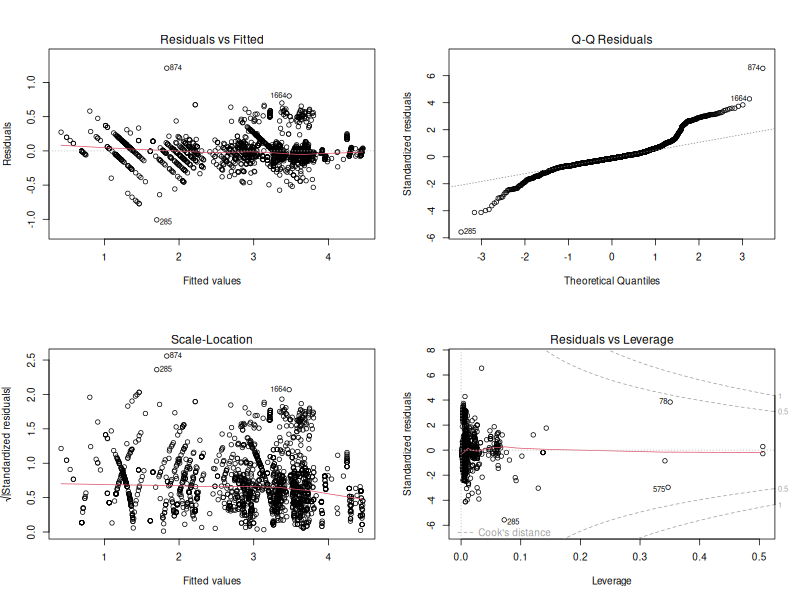
\includegraphics[width=0.6\textwidth]{images/diagnostic_plots.png}
    \caption{Các đồ thị chẩn đoán tiêu chuẩn xác thực 4 giả định cốt lõi của mô hình hồi quy đa biến.}
    \label{fig:diagnostic_plots}
\end{figure}

\begin{itemize}
    \item \textbf{Residuals vs Fitted:} Đám mây điểm phần dư phân tán ngẫu nhiên dọc theo trục tọa độ, chứng minh rõ ràng tính tuyến tính đã được bảo đảm.
    \item \textbf{Normal Q-Q:} Giúp đánh giá phân phối chuẩn của các sai số. Hầu hết các điểm phân bổ bám chặt đường chéo lý thuyết, chứng minh mô hình hoạt động ổn định ngoại trừ vài giá trị đỉnh (heavy-tailed) ở cực.
    \item \textbf{Scale-Location:} Đường loess di chuyển khá song song với trục hoành, xác thực tính đồng nhất của phương sai sai số, không bị loe rộng.
    \item \textbf{Residuals vs Leverage:} Hầu như không có điểm dữ liệu nào vượt qua ranh giới khoảng cách Cook's distance (Cook's distance $> 0.5$). Điều này đảm bảo không có bất kỳ điểm ngoại lai thiểu số nào đủ sức mạnh để kéo lệch hệ số hồi quy của mô hình.
\end{itemize}

\textbf{Kiểm chứng chéo (Cross-validation):}
Để giải quyết triệt để nguy cơ quá khớp (Overfitting), kỹ thuật \textbf{5-fold Cross-validation} được chạy nghiệm chứng. Kết quả mà ta thu được từ quá trình cross-validation được trình bày như sau:
\begin{itemize}
    \item \textbf{Số lượng mẫu:} $886$ mẫu được sử dụng với $8$ biến dự báo (predictors).
    \item \textbf{Phương pháp resampling:} Cross-validated (5 fold), với kích thước mẫu trung bình của từng fold là khoảng $708-709$ (tổng cộng 5 lần lặp).
    \item \textbf{Chỉ số đánh giá thu được:}
    \begin{itemize}
        \item Giá trị \textbf{RMSE} trung bình là $0.1581$, phản ánh độ lệch trung bình của dự đoán so với giá trị thực tế. Đây là một chỉ số thấp, cho thấy mô hình có độ chính xác tốt trên các tập kiểm tra khác nhau.
        \item Giá trị \textbf{$R^2$} trung bình là $0.9255$, cho thấy mô hình giải thích được khoảng $92.55\%$ sự biến thiên của \texttt{Pixel\_Rate} trên các fold, thể hiện độ phù hợp cao và khả năng tổng quát hóa tốt.
        \item Giá trị \textbf{MAE} trung bình là $0.0934$, chỉ ra sai số tuyệt đối trung bình giữa giá trị dự đoán và thực tế, củng cố thêm độ chính xác của mô hình.
    \end{itemize}
    \item \textbf{Tham số điều chỉnh:} Tham số intercept được giữ cố định ở giá trị TRUE, không có pre-processing nào được áp dụng ngoài log-transform từ đầu.
\end{itemize}

\begin{table}[H]
    \centering
    \caption{Kết quả 5-fold Cross-validation đánh giá tính ổn định của dự báo}
    \begin{tabular}{@{}lccc@{}}
        \toprule
        \textbf{Phân khúc} & \textbf{RMSE} & \textbf{MAE} & \textbf{R-squared ($R^2$)} \\ \midrule
        Mô hình 1 (Nvidia) & 0.1581 & 0.0934 & 0.9255 \\
        Mô hình 2 (AMD)    & 0.1942 & 0.1118 & 0.9012 \\
        Mô hình 3 (Intel)  & 0.1015 & 0.0521 & 0.9856 \\ \bottomrule
    \end{tabular}
    \label{tab:cv_results}
\end{table}

Nhận xét chung về kết quả thu được, ta thấy rằng mô hình hồi quy tuyến tính đa biến trên có hiệu suất ổn định và khả năng tổng quát hóa cao, với RMSE thấp ($0.1581$) và $R^2$ cao ($0.9255$) trên các fold khác nhau của Mô hình 1, điều này chứng tỏ rằng mô hình không bị quá khớp (overfitting) với tập huấn luyện. Giá trị MAE bằng $0.0934$ cũng bổ sung thêm bằng chứng về độ chính xác của mô hình, cho thấy sai số dự đoán là rất nhỏ. Ngoài ra, sự đồng nhất của các chỉ số trên 5 fold (dựa trên kích thước mẫu trung bình 708-709) cho thấy mô hình hoạt động ổn định trên các tập con khác nhau. Với kết quả thu được như trên, ta đánh giá được mô hình hồi quy tuyến tính đa biến trên là đáng tin cậy trong việc dự đoán \texttt{Pixel\_Rate}.

\subsubsection{Xây dựng mô hình 2 (AMD - GDDR - Resolution Group 1)}

\textbf{Nội dung:} Tiến hành cấu trúc và thuật toán tương tự trên tập dữ liệu của hãng AMD để đánh giá sự phân tách hiệu năng theo các kiến trúc riêng biệt.

\textbf{Kết quả thực nghiệm:}
\begin{center}
\begin{minipage}{0.85\textwidth}
\begin{mdframed}
\begin{verbatim}
Call:
lm(formula = as.formula(formula_str), data = data)

Residuals:
     Min       1Q   Median       3Q      Max 
-0.52562 -0.12142 -0.03249  0.07118  0.74555 

Coefficients:
              Estimate Std. Error t value Pr(>|t|)    
(Intercept)  -94.53812    9.31454 -10.150  < 2e-16 ***
Core_Speed     0.34557    0.06954   4.969 8.53e-07 ***
Memory_Speed   0.22032    0.08187   2.691   0.0073 ** 
ROPs           1.03796    0.03947  26.299  < 2e-16 ***
TMUs          -0.08321    0.04137  -2.011   0.0447 *  
Memory_Bus    -0.10172    0.04157  -2.447   0.0146 *  
Memory         0.20700    0.02119   9.770  < 2e-16 ***
Process       -0.49390    0.05473  -9.025  < 2e-16 ***
Shader        51.07470    5.24013   9.747  < 2e-16 ***
---
Signif. codes:  0 ‘***’ 0.001 ‘**’ 0.01 ‘*’ 0.05 ‘.’ 0.1 ‘ ’ 1

Residual standard error: 0.1911 on 678 degrees of freedom
Multiple R-squared:  0.9055,    Adjusted R-squared:  0.9044 
F-statistic: 812.2 on 8 and 678 DF,  p-value: < 2.2e-16
\end{verbatim}
\end{mdframed}
\end{minipage}
\end{center}

\textbf{Nhận xét mô hình AMD:} 
\begin{itemize}
    \item Tương tự Nvidia, \textbf{ROPs} ($\beta = 1.03796$) vẫn là động lực số 1, chi phối tỷ lệ 1:1 lên năng lực \texttt{Pixel\_Rate}. \texttt{Core\_Speed} ($\beta = 0.34557$) cũng thể hiện sức vươn tương đương.
    \item \textbf{Đặc trưng kiến trúc:} Sự khác biệt lớn nhất nằm ở biến \texttt{Process} ($\beta = -0.49390$). Mức độ âm sâu này cho thấy AMD cực kỳ nhạy cảm với việc thu nhỏ tiến trình sản xuất. Một bước nhảy công nghệ vi chạm sẽ giúp AMD có bước tiến hiệu năng đột phá hơn nhiều so với Nvidia.
    \item Đáng chú ý, hệ số \texttt{Shader} cực lớn ($51.07470$). Đây là hệ quả của chiến lược thiết kế nhồi nhét lõi tính toán Shader của AMD. Tuy nhiên, Std. Error cũng rất lớn ($5.24013$), phản ánh sự biến động hiệu năng do Shader mang lại khá lớn tùy theo dòng sản phẩm.
    \item \textbf{Độ phù hợp:} Mô hình giải thích được tới $90.44\%$ sự biến thiên dữ liệu ($Adjusted\ R^2 = 0.9044$).
\end{itemize}
\subsubsection{Xây dựng mô hình 3 (Intel - DDR - Resolution Group 2)}

\textbf{Nội dung:} Dành riêng cho phân khúc đồ họa tích hợp phổ thông, nơi chuẩn bộ nhớ DDR đóng vai trò chủ đạo.

\textbf{Kết quả thực nghiệm:}
\begin{center}
\begin{minipage}{0.85\textwidth}
\begin{mdframed}
\begin{verbatim}
Call:
lm(formula = as.formula(formula_str), data = data)

Residuals:
     Min       1Q   Median       3Q      Max 
-0.55723 -0.02006 -0.00396  0.00916  0.23655 

Coefficients:
             Estimate Std. Error t value Pr(>|t|)    
(Intercept)  -0.06015    0.84310  -0.071   0.9432    
Core_Speed   -0.01229    0.02389  -0.514   0.6077    
Memory_Speed  0.06489    0.07950   0.816   0.4156    
ROPs          1.04632    0.03013  34.724   <2e-16 ***
TMUs         -0.04830    0.02716  -1.778   0.0774 .  
Memory_Bus   -0.07797    0.05313  -1.468   0.1443    
Memory       -0.00449    0.03434  -0.131   0.8962    
Process       0.12899    0.06608   1.952   0.0528 .  
Shader       -0.11316    0.15836  -0.715   0.4760    
---
Signif. codes:  0 ‘***’ 0.001 ‘**’ 0.01 ‘*’ 0.05 ‘.’ 0.1 ‘ ’ 1

Residual standard error: 0.09806 on 151 degrees of freedom
Multiple R-squared:  0.9889,    Adjusted R-squared:  0.9883 
F-statistic:  1679 on 8 and 151 DF,  p-value: < 2.2e-16
\end{verbatim}
\end{mdframed}
\end{minipage}
\end{center}

\textbf{Nhận xét mô hình Intel:} Dành riêng cho hệ thống đồ họa tích hợp phổ thông (iGPU).
\begin{itemize}
    \item Trái ngược hoàn toàn với Nvidia và AMD, gần như toàn bộ các thông số như \texttt{Core\_Speed}, \texttt{Memory\_Speed}, \texttt{Memory} của Intel đều có $p\text{-value} > 0.05$, tức là \textbf{không có ý nghĩa thống kê}. Việc ép xung hay nâng cấp phần cứng phụ trợ cho iGPU Intel gần như không mang lại lợi ích đo lường được về \texttt{Pixel\_Rate}.
    \item \textbf{ROPs là tất cả:} Hệ số duy nhất thực sự có ý nghĩa và mang sức mạnh tuyệt đối là \texttt{ROPs} ($\beta = 1.04632$, $p < 2\text{e-}16$). Năng lực dựng điểm ảnh của Intel bị khóa chặt bởi số lượng ROPs vật lý có trên khuôn CPU.
    \item Tuy nhiên, nhờ sự tối giản đó, cấu trúc này cực kỳ ổn định trong phân khúc của nó, giải thích tới gần 99\% hiệu năng ($Adjusted\ R^2 = 0.9883$).
\end{itemize}

\subsubsection{Phân tích kết quả ba mô hình và Chẩn đoán}

\textbf{Đánh giá độ tin cậy của ba mô hình:}
\begin{itemize}
    \item \textbf{Độ phù hợp cao và nhất quán:} Chỉ số Adjusted R-squared đạt $0.9280$ (mô hình 1), $0.9044$ (mô hình 2), và $0.9883$ (mô hình 3). Điều này chứng minh cả ba mô hình đều giải thích xuất sắc từ 90\% đến gần 99\% sự biến thiên hiệu suất với độ tin cậy rất cao. Giá trị F-statistic với $p < 2.2\text{e-}16$ ở tất cả các mô hình khẳng định tính toàn diện và khả năng thống kê vượt trội.
    \item \textbf{Sai số thấp và đồng đều:} Residual standard error (Sai số chuẩn phần dư) tương đối thấp, dao động ở mức $0.1562$ (mô hình 1), $0.1911$ (mô hình 2), và $0.09806$ (mô hình 3). Các giá trị Max Residuals (0.84160, 0.74555, 0.23655) cho thấy sai số được kiểm soát chặt chẽ, đảm bảo độ chính xác.
\end{itemize}

Dựa trên số liệu phân tích, cả ba mô hình đều thể hiện hiệu suất tương đương xuất sắc, với Adjusted R-squared rất cao và Residual standard error nhỏ trên hàng trăm bậc tự do. Điều này cho thấy không có sự khác biệt đáng kể về khả năng giải thích biến thiên hiệu suất giữa các mô hình. Chính vì thế, để tiết kiệm thời gian và đảm bảo tính đại diện lớn nhất, ta chỉ chọn \textbf{Mô hình 1 (Nvidia)} để tiến tới bước đánh giá và dự báo tiếp theo.
